\chapter{Photoluminescence in Silicon Nanoparticles}

Work in this Chapter is adapted from the following papers:
\begin{itemize}
\item Hannah, D.C.; Yang, J.; Podsiadlo, P.; Chan, M.K.Y.; Demortiere, A.; Gosztola, D.J.; Prakapenka, V.B.; Schatz, G.C.; Kortshagen, U.R.; Schaller, R.D. \emph{Nano Letters} \textbf{2012}, 12, 4200
\item Hannah, D.C.; Yang, J.; Kramer, N.J.; Schatz, G.C.; Kortshagen, U.R.; Schaller, R.D. \emph{ACS Photonics} \textbf{2014}, 1, 960
\end{itemize}
\section{Overview}

Although bulk crystalline silicon dominates consumer electronics, the indirect character of its lowest-energy interband transition frustrates utility in optoelectronic devices. Specifically, optical emission and band-edge absorption in this material occurs \emph{via} phonon-assisted transitions between $\Gamma_{\mathrm{valence}}$  and X$_{\mathrm{conduction}}$ symmetries in Brillouin space \cite{hull1999properties}. Because these second-order momentum-conserving processes take place inefficiently, bulk silicon absorbs and emits photons weakly. On the other hand, nanosized silicon structures such as porous silicon \cite{canham1990silicon}, silicon quantum dots formed by self-assembly in SiO2 matrices \cite{shimizu1998optical,zacharias2002size}, and organically terminated colloidally prepared nanocrystals (NPs - as we study both amorphous and crystalline particles later in this Chapter, we utilize the abberviation "NP" rather than "NC" for the duration of this Chapter) \cite{mangolini2007plasma,erogbogbo2010vivo,mangolini2005high,pettigrew2003solution,hessel2011synthesis,holmes2001highly,atkins2011femtosecond} exhibit significantly enhanced emission efficiencies with PL (PL) quantum yields that can exceed 50\% \cite{PhysRevB.80.115407,jurbergs2006silicon,Wilson19111993}.  While the high PL efficiencies invite applications in nontoxic biolabeling \cite{erogbogbo2010vivo} and energy-efficient light-emitting diodes \cite{ng2001efficient,cheng2011high} the mechanisms and origin of bright PL in nanosized silicon have remained a subject of discussion for more than two decades \cite{canham1990silicon, PhysRevB.49.16845,PhysRevLett.88.097401,reboredo2005theory,
de2010red,PhysRevB.61.4485,cullis1991visible,PhysRevLett.100.067401,saar2009PL,kovalev1999optical,PhysRevLett.72.1514,PhysRevLett.81.2803, godefroo2008classification}. \par

Silicon nanocrystals generally exhibit both a high-energy and low-energy photolumiscence band. Reports vary considerably in the origins attributed to each band and even more so in the timescales reported for the lifetime of each band, which span the picosecond to microsecond timescales. Relevant previous work related to each PL band will be discussed below. In this Chapter, we report the pressure-dependent PL from plasma grown, alkane-terminated colloidal particles. We find a systematic PL red shift that matches the X$_{\mathrm{conduction}}$-to-$\Gamma_{\mathrm{valence}}$ transition of bulk crystalline silicon. These results, reinforced by calculations, suggest that efficient PL, frequently attributed to defects, arises instead from core-states that remain highly indirect despite quantum confinement. \par

We also examine ultrafast, high-energy PL produced from such Si nanocrystals as a function of both particle size and lattice crystallinity. In particular, we quantify the decay time and spectral profiles of nominally few-picosecond direct-gap emission previously attributed to phononless electron-hole recombination. We find that the high-energy (400-600 nm, 2-3 eV) PL component consists of two decay processes with distinct time scales. The fastest PL exhibits an $\sim$30 ps decay constant largely independent of emission energy and particle size. Importantly, nearly identical temporal components and blue spectral features appear for amorphous particles. We thus associate high-energy, rapid emission with an amorphous component in all measured samples, as supported by Raman analysis and MD simulation. Based on these observations, we advise that the observed dynamics proceed too slowly to originate from intraband carrier thermalization and instead suggest a nonradiative origin associated with the amorphous component.

\section{The Origin of Long-Lived, Low-Energy Photoluminescence in Si Nanoparticles}

High surface-to-volume ratios, broad particle size distributions, extrinsic effects of encapsulation matrices and material defects, together with complex PL recombination dynamics, all contribute to a lack of consensus regarding the origin of PL in nanosized silicon. Overall, two origins largely govern the discussion \cite{saar2009PL}.  First, a quantum confinement model, well-known to accurately describe properties of several direct-gap nanomaterial compositions, invokes disruption of the stringent relationships between carrier energy and translational momentum as electronic density of states (DOS) becomes discrete for particle sizes comparable to or smaller than the exciton Bohr radius ($\sim$4.2 nm). Such confinement effects can greatly enhance electron-hole recombination and may impart direct gap character to the lowest-energy electronic transitions \cite{PhysRevLett.72.1514}, which would bolster optoelectronic applications. The quantum-confinement model draws support from observations of characteristic-phonon-assisted PL \cite{PhysRevLett.81.2803}, fast (nanosecond) decay times \cite{PhysRevLett.100.067401,english2002size,kusova2010brightly,groenewegen2010excited}, correlations of particle size with emission energy \cite{Wilson19111993,kovalev1999optical,english2002size,mastronardi2011preparation}, and sensitivity of PL spectra to large magnetic fields \cite{godefroo2008classification}.  The second model instead attributes the high-efficiency PL to surface states wherein any quantum-confined core states that may exist do not produce substantial emission. Instead, excited carriers rapidly relax into lower-lying defect states that slowly radiate \cite{PhysRevB.49.16845,PhysRevLett.88.097401,godefroo2008classification,PhysRevLett.100.067401,PhysRevLett.76.2961,PhysRevB.48.11024,PhysRevB.84.085321}. In this model, chemical details of the crystal surface termination, such as varied abundance and distributions of surface moieties, as well as surface reconstructions, yield tuning of the emission energy largely independently of any particle core-states. Experimental support for the surface-state model arises from observables such as broad emission spectra, sensitivity to chemical treatments \cite{PhysRevLett.82.197}, insensitivity of PL spectra to large magnetic fields \cite{godefroo2008classification}, and long-lived PL decay features (microseconds time scale) \cite{PhysRevLett.100.067401,PhysRevLett.82.197,vzidek2010femtosecond}, which seem inconsistent with the discrete translational-momentum-relaxed DOS of quantum-confined core states. \par

In this thesis, we examine both X-ray diffraction (XRD) and PL as functions of pressure imparted using a diamond anvil cell for multiple samples of highly crystalline, plasma-synthesized, alkane-terminated colloidal Si NPs with the goal of obtaining insights regarding the origin of the efficient PL. From XRD, we first determine the diamond-phase bulk modulus of multiple Si NP sizes and find that obtained moduli closely match the bulk constant in distinction from NPs formed from binary semiconductors \cite{jiang2004phase}. We also observe several crystal phases including Si(I), Si(V), Si(VII), and amorphous Si (a-Si). The structural studies are reported in the following Chapter. In this Chapter, we focus on optical characterization. In pressure-dependent PL studies, we find that in all cases the emission energy closely follows the pressure-dependence of the bulk-phase, band-edge deformation potential associated with the X-to-$\Gamma$ transition. Taken together, this data clearly indicates that the long-lived but efficient PL arises from core-states with indirect-gap character rather than from surface states in these samples. Lastly, we show from calculations that the energy shift is consistent with delocalized NP-core band-edge states using a combination of MD for pressurization and DFT for electronic properties, regardless of the presence or absence of a common oxide surface defect.  

\subsection{Plasma Synthesis of Si Nanoparticles}

The Si NPs studied here were fabricated by room-temperature plasma dissociation of SiH$_4$ using a system described previously \cite{mangolini2007plasma}. A mixture of SiH$_4$/He (5\%/95\% by volume) and argon was introduced into a quartz 13.56 MHz radio frequency (30-100 W) plasma reactor with 6.3 mm inner diameter and 9.5 mm outer diameter, at flow rates of 13 and 35-100 standard cubic centimeters per minute (sccm), respectively. Variation of the plasma power permits tunability of the Si NP crystallinity from highly amorphous to highly crystalline.  Highly crystalline samples were utilized in all pressure-dependent experiments.  The properties of less crystalline and amorphous particles will be explored in later sections of this thesis. An additional H$_2$ flow (100 sccm) was injected at the end of the plasma region to initially H-terminate the NP surfaces. NP size was controlled by particle collection pressure and examined by XRD. Indicated NP radii result from Scherer analysis of diffraction peaks. The Si NPs were collected on mesh filters and then ultrasonicated to obtain a suspension in a mixture of 1-dodecene ligand and mesitylene solvent with a ratio of 1:5 by volume with a specific volume of 3.3 mL of mesitylene per milligram of NPs. The suspension was transferred into a flask reactor and refluxed under N$_2$ flow at 215 $^{\circ}$C. Surface functionalization with dodecane was indicated by transformation of an initially cloudy suspension into a clear solution. The NPs were dried under vacuum at 150 $^{\circ}$C and redissolved in hexane. All steps were carried out in an inert nitrogen-gas environment. PL quantum yields were measured using a silicon CCD, a 400 nm light-emitting diode excitation source, and integrating sphere.

\subsection{Pressure-Dependent Photoluminescence in Si Nanoparticles}

\subsubsection{Experimental Details}
Si NPs were dissolved in ethylcyclohexane and loaded into a diamond anvil cell under a nitrogen atmosphere. A small ruby crystal was placed in the pressure cell along with the NP solution for independent determination of applied pressure \emph{via} ruby R1 fluorescence. PL spectra were produced by exciting at 473 nm with a continuous-wave laser through a long-working distance 10$\times$ objective. The same objective collected PL and directed PL photons to a 300 mm spectrograph outfitted with liquid nitrogen-cooled silicon and InGaAs array detectors. Time-correlated single photon counting (TCSPC) was produced using a 2 kHz, 405-nm laser diode, grating spectrograph, and avalanche photodiode.
\subsubsection{Basic Characterization of Plasma-Synthesized Si Nanoparticles}
Figure \ref{f:sipressure1}(a) shows static PL spectra collected for different NP samples at ambient pressure. XRD-derived NP sizes decrease with increasing PL energies as generally expected for a quantum-confined semiconductor. For the bluest-emitting NP sample, we note that the PL energy is $\sim$38\% higher than the bulk-phase energy gap. All measured samples exhibited quantum yields in the tens of percent range. TCSPC for the samples showed that the efficient PL signals arise due to slow radiative processes, characterized in Figure \ref{f:sipressure1}(b) as exhibiting a fairly single exponential decay with a 75.8 ($\pm$0.3) $\mu$s lifetime. Furthermore, transmission electron microscopy, selected area electron diffraction, and XRD each indicated highly crystalline particles (Figure \ref{f:sipressure1}(c)). Transmission electron microscopy confirmed the average particle sizes determined by XRD and established a particle size dispersion of $\sim$20\% for each of the samples examined herein. \par

\begin{figure}
\begin{center}
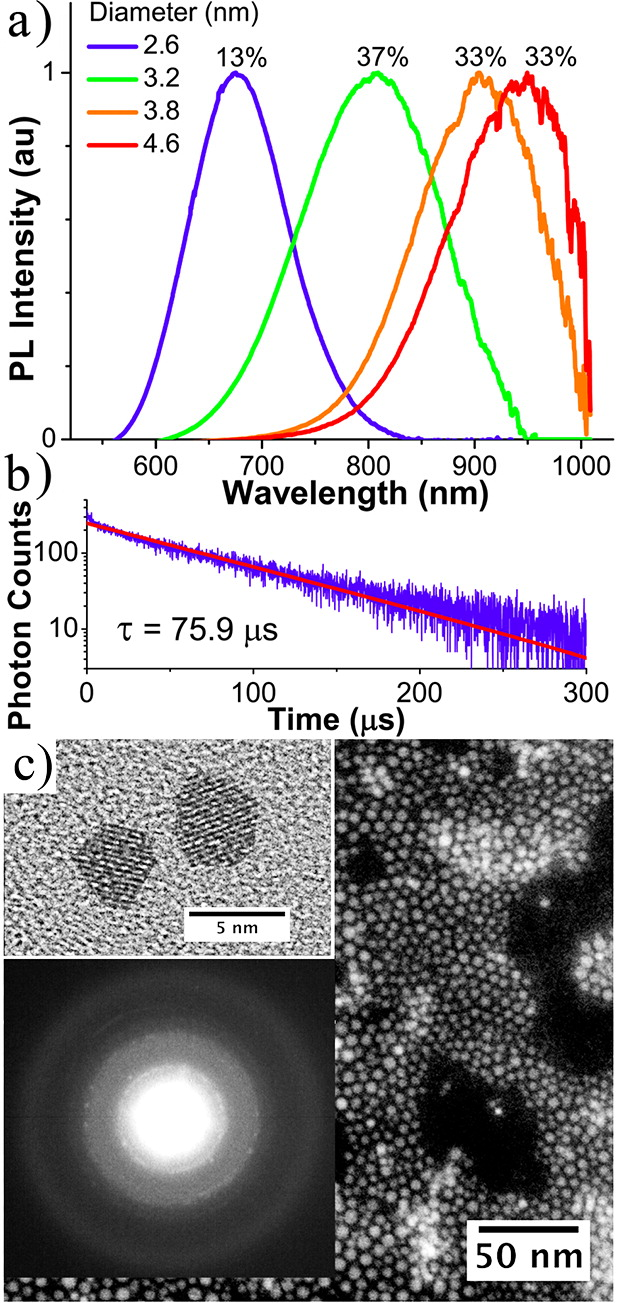
\includegraphics[width=0.35\textwidth]{./Chapter6/sipressure1.jpeg}
\caption[Basic characterization of various sizes of plasma-synthesized Si NPs.]{(a) Ambient pressure PL spectra of silicon NPs with indicated average NP diameters and PL quantum yield. Loss of detector sensitivity beyond 1020 nm artificially influences the largest NP sample spectrum. (b) Time-correlated single photon counting of a 2.6 nm diameter NP sample at ambient pressure measured at 680 nm shows a highly single-exponential decay with a 75.8 $\mu$s lifetime. (c) Transmission electron micrographs of the 3.2 nm sample (main panel). The high-resolution TEM image in the upper inset shows high crystallinity that is also apparent in selected area electron diffraction (lower inset).}
\label{f:sipressure1}
\end{center}
\end{figure}

\subsubsection{Optical Properties of Si Nanoparticles Under Pressure} 
Substantial structural characterization of Si NPs at elevated was performed, the details of which are reported in the following Chapter.  Here, we focus on characterization of the optical properties of the NPs as a function of applied pressure.  Figure \ref{f:sipressure4}(a) displays spectrally resolved PL of the 2.6 nm diameter Si NPs for a range of hydrostatic pressures.  For each pressure, the PL spectrum appears Gaussian with a clearly identifiable emission maximum. Here, increasing pressure produces a distinct red shift of the PL as well as a reduced integrated intensity. Figure \ref{f:amsi4}(b) plots the PL centroid calculated from the data in Figure \ref{f:amsi4}(a) as well as similar measurements performed for the other three Si NP samples. In addition, we plot trend lines for the bulk phase derived from literature sources \cite{PhysRev.98.1755, slykhouse1958effect}.  Linear fitting of the PL emission maximum versus pressure for the different samples yields values of -17.2, -14.2, -21.1, and -21.3 meV/GPa for mean particle diameters of 2.6, 3.2, 3.8, and 4.6 nm, respectively. These band gap dependences on pressure were independent of pressure change direction showing no hysteresis provided that we did not exceed the phase transition near $\sim$20.5 GPa. The observed PL energy dependences on pressure closely agree between samples and also agree with the reported values of −15 and −20 meV/GPa for the band gap of bulk silicon \cite{PhysRev.98.1755, slykhouse1958effect, welber1975dependence}. 

\begin{figure}
\begin{center}
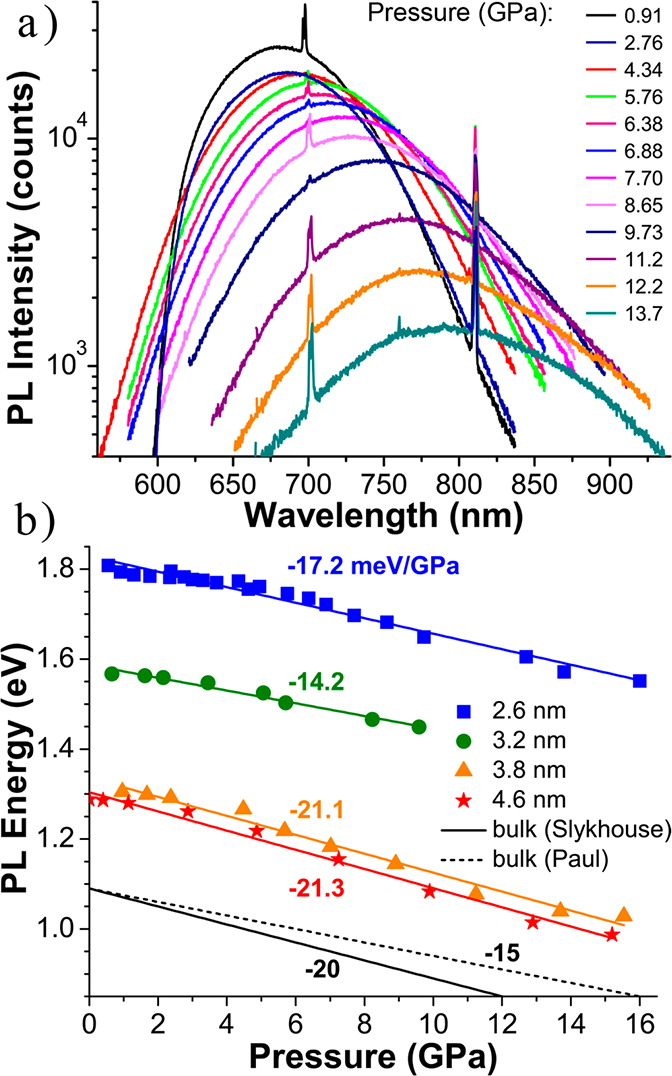
\includegraphics[width=0.5\textwidth]{./Chapter6/sipressure4.jpeg}
\caption[Pressure-dependent PL spectra of plasma-synthesized Si NPs.]{PL spectra of 2.6 nm diameter Si NPs exhibit a red shift as a function of applied pressure. Ruby R1 fluorescence gives rise to the narrow spectral feature near 700 nm and second-order diffraction of the excitation laser produces the narrow feature near 810 nm.  (b) The PL centroid emission energy as a function of pressure for all samples exhibits a shift to lower energy with pressure and closely follows the dependence exhibited by bulk silicon taken from two different sources \cite{PhysRev.98.1755, slykhouse1958effect}.}
\label{f:sipressure4}
\end{center}
\end{figure}

In crystalline semiconductors, compression of the bulk-phase crystal lattice induces energetic changes in band positions. In bulk silicon, the band-edge X$_{\mathrm{conduction}}$-to-$\Gamma_{\mathrm{valence}}$ transition red shifts with increasing pressure while the higher-energy $\Gamma$-to-$\Gamma$ direct-gap blue shifts. The lowest-energy “band-edge” transition arises from two terms in quantum-confined systems corresponding to the bulk energy gap, $E_{bulk}$, plus a quantum-confinement energy term, $E_{QC}$, related to the particle size in comparison to the exciton Bohr radius. In the pressure range examined for the optical studies, NP-volume reduction upon compression imparts negligible changes in radius (at 15 GPa the particle is still $\sim$89\% of its ambient pressure volume, so $<$4\% change in radius) and thus negligible changes in quantum confinement energy. However, the bulk deformation potential produces large changes in the lowest-energy transition \emph{via} the $E_{bulk}$ contribution as reflected in the bulk-phase pressure dependence (Figure \ref{f:sipressure4}(b)). By contrast, surface states are expected to form highly localized excitations that would yield less sensitive dependence of PL energy on pressure. The concurrence of both the sign and amplitude of the pressure-dependent PL shift together with the size-independent bulk modulus of silicon suggests a core-derived origin for the emitting state in these Si NPs. In the range of NP sizes studied, our measurements provide evidence that the efficient PL from Si NPs arises from the X$_{\mathrm{conduction}}$-to-$\Gamma_{\mathrm{valence}}$ indirect transition despite substantial quantum confinement, consistent with the interpretation provided by Brus \cite{Wilson19111993}.  \par

To substantiate the claim that the observed pressure dependence of the PL peak originates from bulk-like Si states rather than surface moieties, we present pressure-dependent DFT calculations of energy gap for a model Si NP.  Specifically, we used the Vienna Ab Initio Simulation Package (VASP) \cite{PhysRevB.54.11169} with supplied Projector Augmented Wave potentials \cite{kresse1999ultrasoft} for core electrons.  A 2 nm diameter, hydrogen-passivated, faceted Si nanocrystal was constructed from known surface energies of H-passivated Si (100), (110), and (111) surfaces \cite{hong2000equilibrium} using the Wulff construction. For each pressure, the model H-terminated Si NP \cite{PhysRevB.37.6991} is compressed by hydrostatic pressure using an inert fluid comprising 108 000 particles with classical MD (MD) methods \cite{martovnak2002pressure}, and the energy gap between the highest occupied and lowest unoccupied molecular orbitals (HOMO and LUMO, respectively) was then calculated using DFT for 11 images within the MD trajectory. Further details regarding these calculations can be found in Appendix D. The effect of a common surface defect, a Si-O-Si, was also investigated and the results are shown in Figure \ref{f:sipressure5}(a,b). We find that the HOMO-LUMO gap of the Si NP decreases linearly with increasing pressure, as observed in the experiment, regardless of the presence or absence of the surface defect group. Charge density iso-surfaces for the HOMO and LUMO at pressures of 1 and 20 GPa are shown in Figure \ref{f:sipressure5}(c,d). We see that the HOMO and LUMO are extended and not localized on the surface, regardless of existence of the surface defect. \par

\begin{figure}
\begin{center}
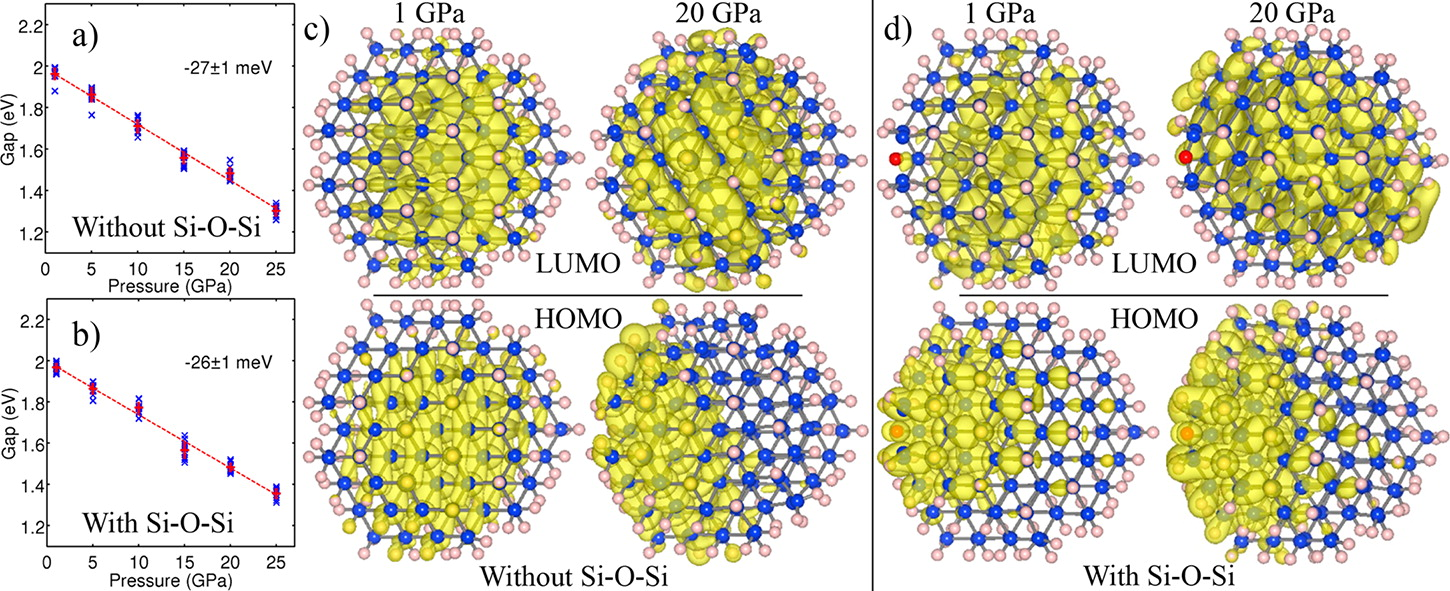
\includegraphics[width=\textwidth]{./Chapter6/sipressure5.jpeg}
\caption[Pressure-dependent energy gap of Si NPs derived from density functional theory.]{Pressure dependence of the HOMO-LUMO energy gap in a 2 nm diameter model H-passivated Si NP (a) without and (b) with a surface defect group (Si-O-Si). At any given pressure, blue crosses ($\times$) denote the HOMO-LUMO gaps for the NP at different steps in the MD trajectory, while the red plus symbol (+) denotes the mean gap. The red dashed line is a linear fit to the mean gaps with the indicated slope. HOMOs and LUMOs for the model Si NP under hydrostatic pressures of 1 and 20 GPa for the NP (c) without and (d) with a surface defect group (Si-O-Si).}
\label{f:sipressure5}
\end{center}
\end{figure}

\subsubsection{Conclusions}
In conclusion, we used pressure to investigate the origin of efficient PL in alkane-terminated, plasma-synthesized Si NPs. We showed that both the bulk modulus and PL emission feature of the investigated NPs shift in step with the bulk crystalline material. These findings strongly suggest that the bright emission from these alkane-terminated Si NPs originates from the X-to-$\Gamma$ transition with insignificant mixing from other bands in the size-range examined. Overall, the indirect-gap character present in the bulk phase remains dominant despite the expectation of relaxation between carrier energy and momentum as quantum-confinement imparts discretization of DOS. The radiative recombination from core-states remains long-lived despite the up to 38\% contribution from quantum confinement to the overall NP emission energy examined here. Finally, because the efficient PL originates from the core states in these structures, our results suggest that optimization of the emission quantum yield from Si NPs, like many other compositions, relies upon surface passivation with ligands that lack density of states within the energy gap rather than decoration of the surface with efficiently emitting surface traps.

\subsection{In Silicon Nanoparticles, Ultrafast Visible-Light Photoluminescence Arises from a Ubiquitous Amorphous Shell}
As noted above, nano-sized Si often exhibits 10\% or greater quantum yield with reported decay components spanning microsecond to picosecond time scales \cite{PhysRevLett.100.067401,de2010red,english2002size,kusova2010brightly,groenewegen2010excited,PhysRevB.49.16845,PhysRevLett.88.097401,godefroo2008classification,PhysRevB.84.085321,dohnalova2013surface}. However, despite numerous studies, disagreement exists regarding the origin of both the fast and slow decay processes. The 650-1000 nm PL feature (termed throughout this section as the “red” feature) displays a microsecond lifetime, and was found in the previous section to originate from indirect gap (X$_{\mathrm{conduction}}$-to-$\Gamma_{\mathrm{valence}}$) recombination.  In this section, we focus on characterization of the radiative recombination that occurs in the 400 to 600 nm energy range, referred to herein as the “blue” feature. \par

Significant excitement exists with regard to multiple reports of fast (nanosecond to subnanosecond) 400 to 600 nm (2-3 eV) PL decay features in Si NPs \cite{PhysRevLett.100.067401,de2010red,dohnalova2013surface,tsybeskov1994blue,valenta2008origin}. Observations of such blue emission, which appear for both Si NPs produced \emph{via} wet chemical synthesis \cite{yang1999synthesis,holmes2001highly}, as well as for plasma-grown materials \cite{PhysRevLett.100.067401} are often attributed to emergent direct gap optical transitions \cite{PhysRevLett.100.067401,de2010red,valenta2008origin} that may arise from at least two possible mechanisms. First, the bulk semiconductor requirement of carrier energy and linear momentum conservation can become less stringent upon quantum-confinement owing to replacement of electronic band structure with discrete electronic states, in similarity to molecules \cite{PhysRevLett.101.217401,PhysRevLett.75.3728}. In addition, during the time that a photoexcited electron and hole (an exciton) collectively exceed the lowest energy “band-edge” transitions ($\sim$1 ps in most semiconductor nanomaterial compositions) \cite{PhysRevLett.80.4028,PhysRevLett.95.196401}, radiative recombination can occur between states that possess the same momentum and do not necessitate involvement of a momentum-conserving phonon \cite{de2010red}. Observation of such “phononless” emission from hot exciton states requires either large oscillator strength or slowed cooling of hot excitons. \par

A recent report utilized time-resolved PL spectroscopy and a quasi-continuous sample re-excitation scheme in order to accentuate and spectrally characterize blue emission features, but lacked sufficient time-resolution to directly characterize the time scale of the recombination process \cite{de2010red}. An additional study also suggested that direct-gap transitions may arise in colloidally prepared, alkyl-terminated NPs owing to modification of the electronic structure by covalent surface functionalization \cite{dohnalova2013surface}. In this case, 400-600 nm emission does not compete with intraband relaxation, but instead, hybridization with the covalently attached surface ligands purportedly modifies the band-edge electronic wave functions such that substantial broadening of the related $k$-space distribution occurs, permitting direct recombination at the $\Gamma$-point. That report concludes that high-energy emission stems from recombination produced within the Si NPs rather than from defect states, but the dynamics of the obtained PL spectra were not characterized with sufficient time-resolution to distinguish processes related to carrier thermalization. \par

Here, we examine multiple sizes and degrees of crystallinity of plasma-synthesized colloidal Si NPs using a previously reported synthetic method \cite{PhysRevB.80.115407} with a focus on emission in the 400-600 nm “blue” spectral region. We spectrally and, for the first time, temporally resolve PL from the particles with up to single-picosecond time resolution. From these measurements we observe a $\sim$30 ps decay component as the fastest PL relaxation time scale. This spectral and temporal resolution allows us to definitively assign lifetimes to the observed PL features. Based on our observations, we suggest that the blue PL band in Si NPs originates from an amorphous component in the samples and that the rapid emission processes are too slow to be consistent with a hot exciton radiative process. We also show through MD (MD) simulations that experimental Raman spectra obtained at different plasma powers are well-described by particles presenting a thin, amorphous surface (consistent with electron microscopy) which we suggest gives rise to the fast emission.

\subsubsection{Transient Photoluminescence Experiments}
Alkyl-passivated Si NPs fabricated using the synthesis method detailed above and in the work by Mangolini \emph{et al.} \cite{mangolini2007plasma} were suspended in octane and loaded into an airtight cuvette under a nitrogen atmosphere. The room-temperature NPs were photoexcited with 35 fs pulses from a 2 kHz amplified Ti-sapphire laser at 325 nm (3.8 eV). Excitation fluence sufficient to ensure single exciton dynamics ($N_{exc} << 1$) was utilized. PL photons were directed to a 150 mm spectrograph and single-photon-sensitive streak camera. Detector regions were binned vertically or horizontally to produce time-resolved spectra or spectrally resolved dynamics, respectively. It is important to note that the time resolution of a streak camera inherently depends on the observation window. Longer observation windows necessarily yield reduced temporal resolution, and vice versa. Therefore, dynamics which appear well-resolved by a streak camera utilizing a 120 ps observation window can appear instrumentally limited when examined using longer observation windows.

\subsubsection{Ultrafast Photoluminescence Dynamics of Highly Crystalline Silicon (c-Si) Nanoparticles}
Crystalline Si-NPs were synthesized in a radio frequency (RF) plasma (80 W) and covalently functionalized with 1-dodecane using the methods described above. Single-exciton PL dynamics under ambient conditions were examined using a streak camera, which provides simultaneous spectral and temporal resolution as described above. Figure \ref{f:amsi1} (left panel) depicts a streak camera image of PL recorded for the first 10 ns following photoexcitation of an ensemble of 3.2 nm-diameter crystalline Si (c-Si) NPs. The top right panel of Figure \ref{f:amsi1} shows a late-time PL spectrum (temporally integrated from 9-10 ns), which reveals two clear contributions: a blue PL band centered near 450 nm and a red PL band centered at 700 nm. The presence of distinct blue and red bands is consistent with many previous reports \cite{PhysRevLett.100.067401,tsybeskov1994blue,valenta2008origin,yang1999synthesis,holmes2001highly}, although their origins remain disputed. PL immediately following the excitation pulse (integrated from 0-1 ns, shown in the bottom right panel of Figure \ref{f:amsi1}) reveals a third PL band intermediate in energy, termed the “green” feature. Such a green feature was reported by de Boer \emph{et al.}, who attributed it to phononless radiative recombination of hot excitons, despite a lack of direct dynamical characterization \cite{de2010red}. \par

\begin{figure}
\begin{center}
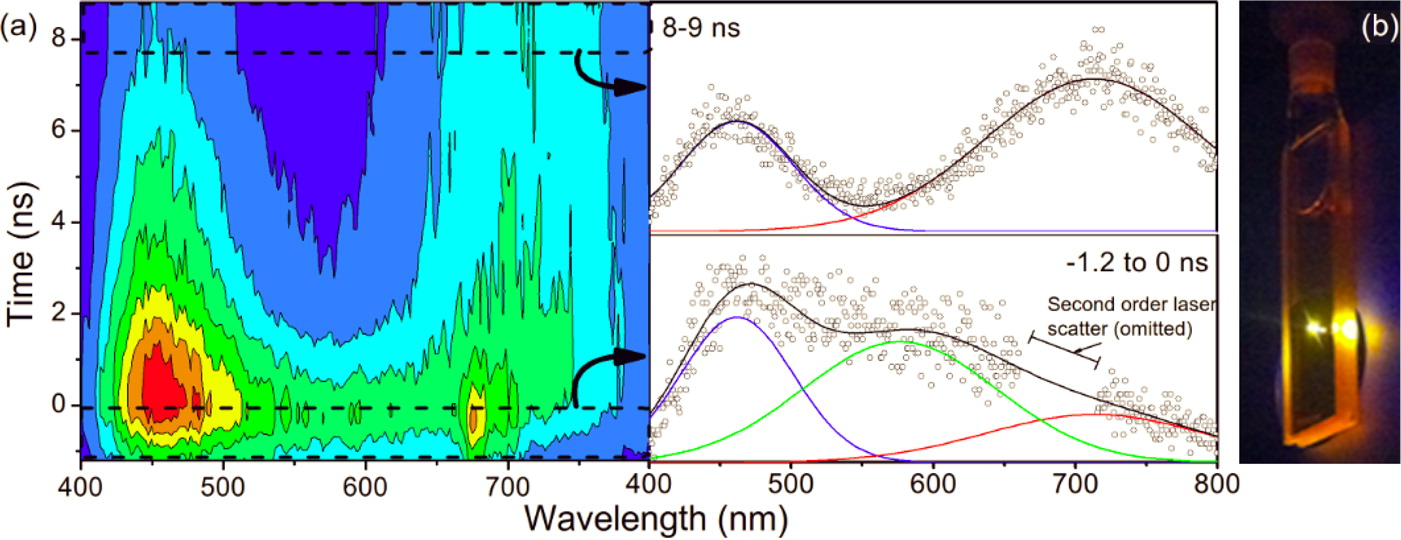
\includegraphics[width=\textwidth]{./Chapter6/amsi1.jpeg}
\caption[Nanosecond-scale evolution of PL from crystalline Si nanoparticles.]{(a) A streak camera image for crystalline 3.2 nm diameter Si NPs photoexcited at 325 nm (3.8 eV). Dynamics over a 10 ns time window subsequent to photoexcitation are shown. The apparent buildup of PL prior to $t = 0$ is related to an instrumentally limited response. The panels on the right side show PL spectra integrated temporally over the regions indicated by the dotted lines and arrows in the left panel (top right panel: PL spectra from 9-10 ns, bottom right panel: 0-1 ns). Solid lines in the right panels indicate Gaussian lineshapes used to fit the PL spectra. The peak centers and line widths obtained from the fits in the 9-10 ns spectra were fixed and used in the fitting of the 0-1 ns spectra, a procedure justified by the absence of temporal evolution in the PL line width. In the bottom right panel, data points from 650-700 nm are contaminated by second order scatter from the 325 nm excitation source; these points are omitted from the plot and the Gaussian fitting procedure. (b) A photo showing PL from 3.2 nm diameter Si NPs.}
\label{f:amsi1}
\end{center}
\end{figure}

To investigate the fast dynamics of these features we examined PL using single-picosecond temporal resolution streak camera electronics. Such high time resolution measurements applied to a broadband emitter necessitate the use of bandpass spectral filtering in order to obtain wavelength-resolved dynamics free from artifacts. Figure \ref{f:amsi2}(a) depicts a streak camera image of PL from the same ensemble of 3.2 nm diameter c-Si NPs for 100 ps following photoexcitation. Because of required filtering optics, only the high-energy shoulder of the red PL band is observed and the high-energy edge of the blue PL band is also truncated. Truncation due to filtering optics is indicated in Figure \ref{f:amsi2}(a). The red feature exhibits a microsecond decay lifetime and is present in this data as a persistent shelf. The blue feature, however, exhibits decay on this time scale; this is evident in the time-resolved spectra displayed in Figure \ref{f:amsi2}(b) for the same sample. Notably, aside from decreasing intensity with time, the spectra exhibited little temporal evolution in terms of both energy and spectral profile. For all c-Si NP sizes studied, the PL spectral profile remains relatively constant for 800 ps following photoexcitation. Importantly, the consistent PL profile at blue wavelengths suggests that the decay in PL intensity is due to the collective depletion of a single population of emitters. We explore the blue feature dynamics further in Figure \ref{f:amsi2}(c), which displays PL intensity at 500 nm as a function of time for the same sample. Comparison to the instrument response function (IRF, also shown in Figure \ref{f:amsi2}(c)) obtained from examination of pump laser scatter indicates that the blue feature decay is well-resolved at these time scales and that no faster dynamics are taking place in the system with significant amplitude. Fitting the dynamics in Figure \ref{f:amsi2}(c) to a monoexponential decay function yields a time constant of 28 ps. At slightly longer times, a subnanosecond decay component is also observed. Fitting the dynamics from 0 to 800 ps to a biexponential decay function yields time constants corresponding to the $\sim$30 ps feature discussed above and a component having a lifetime that is consistently hundreds of picoseconds (see Table \ref{table:amsiT1} for fitting results and Appendix C for PL dynamics from 0-800 ps). \par

\begin{figure}
\begin{center}
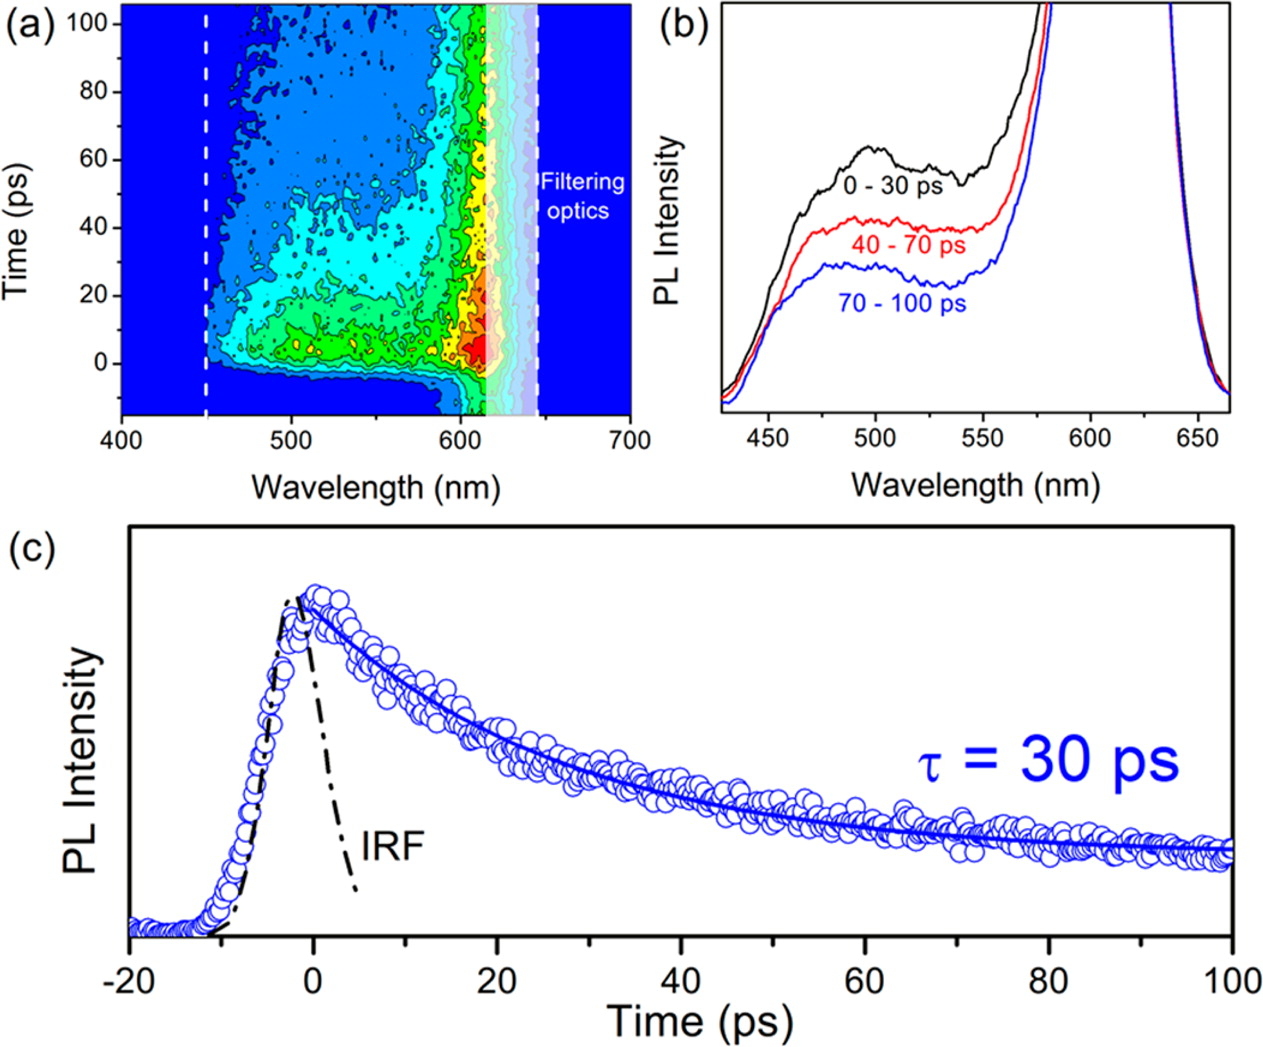
\includegraphics[width=0.75\textwidth]{./Chapter6/amsi2.jpeg}
\caption[Picosecond-scale evolution of PL from crystalline Si nanoparticles.]{(a) Streak camera image of PL from the 3.2 nm diameter Si NPs recorded for 100 ps following photoexcitation. Necessary filtering optics and sample reabsorptions artificially truncate the PL spectrum on the red and blue edges. Truncation due to band-pass filtering is indicated by dashed white lines, while the translucent white shading indicates regions where signal is attenuated by the filtering optics, but not completely blocked. The high-energy tail of the red PL band is apparent as a long-lived shelf, as it does not fully relax prior to re-streaking of the time-resolving detector. (b) Main panel: Time-resolved PL spectra in three different temporal regions for the same sample. Temporally binned regions are indicated by labels. (c) Time-resolved PL dynamics spectrally integrated from 475 to 525 nm. The solid blue line indicates a fit of the dynamics to a single exponential decay function. The instrument response function (IRF) is indicated by a dotted black line. Note that this IRF corresponds only to a streak camera observation window of 120 ps.}
\label{f:amsi2}
\end{center}
\end{figure}

\begin{table}
\caption{Time Constants for the Biexponential Decay Observed in the PL Dynamics for the First 800 ps Following Photoexcitation of 4 Silicon NP Sizes.$^a$}
\centering
\begin{tabular}{c r r }
\hline\hline
Diameter (nm) & $\tau_1$ (ps) & $\tau_2$ (ps) \\
\hline
2.6 & 27.8 $\pm$ 0.6 & 204 $\pm$ 7 \\
3.2 & 26 $\pm$ 4 & 243 $\pm$ 12 \\
3.8 & 16 $\pm$ 1 & 195 $\pm$ 13 \\
4.6 & 26 $\pm$ 7 & 563 $\pm$ 47 \\
\hline
\end{tabular} \par
\bigskip
$^a$ Errors are derived from the fitting function.
\label{table:amsiT1}
\end{table}

Notably, picosecond scale dynamics do not reveal distinct blue and green decay components, indicating that the green feature noted in Figure \ref{f:amsi1} displays dynamics that are indistinguishable from the blue feature on picosecond time scales, and that no spectral range exhibits decay dynamics having a time constant faster than $\sim$20 ps.

\subsubsection{Characterization of Amorphous Silicon Nanoparticles}
In addition to highly crystalline particles, we examined reduced crystallinity Si NPs produced using lower plasma power as described and characterized in depth in recent reports \cite{PhysRevB.80.115407,anthony2011routes}. Noting numerous reports of visible PL from amorphous silicon structures \cite{pankove1977PL, wang2003high,wehrspohn1997electrochemistry}, we systematically investigated the role of lattice crystallinity on PL spectrum. Figure \ref{f:amsi3}(a) depicts Raman scattering collected from Si NPs synthesized at plasma powers of 8, 30, 45, and 60 W. NPs synthesized at higher powers clearly yield more narrow Raman scattering spectra, consistent with higher crystallinity samples. The NPs synthesized at 8 W exhibit a broad, featureless peak, corresponding to an entirely amorphous sample \cite{PhysRevB.80.115407}. We also present the Raman scattering spectrum of bulk crystalline Si, which exhibits a sharp peak at 520 cm$^{-1}$ corresponding to the transverse optical (TO) phonon mode. This peak is also clearly present in the Si NP Raman scattering spectra, along with a low-frequency shoulder, the presence of which has been correlated with amorphous materials \cite{duan2012raman}. The relative intensity of the low-frequency shoulder appears to be larger for lower plasma powers.

\begin{figure}
\begin{center}
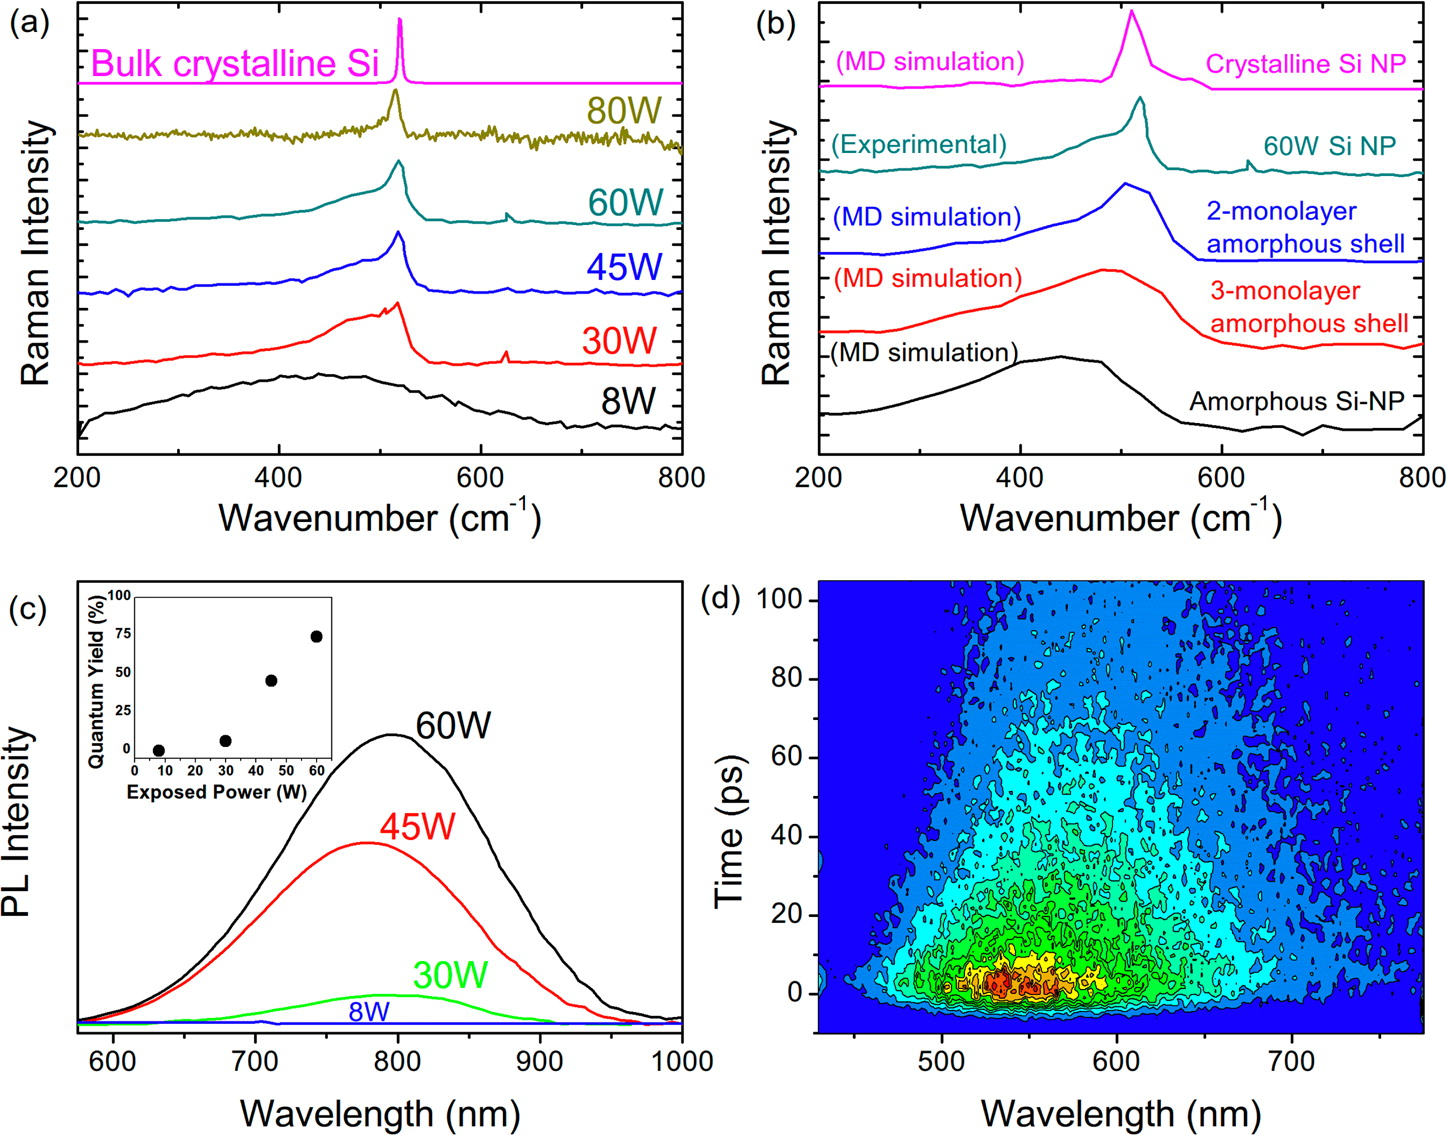
\includegraphics[width=0.75\textwidth]{./Chapter6/amsi3.jpeg}
\caption[Raman scattering and PL from Si NPs synthesized at a variety of powers.]{(a) Raman scattering spectrum of Si NPs synthesized at the indicated plasma powers. The peak at 500 cm$^{-1}$ is attributed to the transverse optical (TO) phonon and diminishes in intensity for samples synthesized at lower powers (less crystalline). The Raman scattering spectrum of bulk crystalline Si is also displayed. All Raman spectra have been mathematically normalized and plotted with a vertical offset. (b) Raman scattering spectra for Si NPs predicted from MD simulations as described in the Appendix. Color-coded data is shown for a fully crystalline particle, particles with 2 or 3 monolayers of amorphous Si on their surfaces, and a fully amorphous particle. The experimental data for Si NPs synthesized at 60 W from (a) is reproduced here for comparison. (c) PL spectra of Si NPs synthesized at four different plasma powers (indicated on the figure). Higher plasma powers nominally yield more crystalline samples. Inset: PL quantum yield for Si NPs as a function of the plasma power used during their synthesis. (d) A streak camera image of PL from Si NPs synthesized at a plasma power of 8 W (e.g., fully amorphous Si). Photoexcitation energy was 3.8 eV.}
\label{f:amsi3}
\end{center}
\end{figure}

To gain a clearer understanding of the correspondence between Raman spectra, sample crystallinity, and address the potential coexistence of crystalline and amorphous phases, we performed MD simulations of experimentally sized (4 nm diameter) Si NPs that present varying amounts of amorphous material on the surface. The construction of particles presenting an amorphous surface was motivated by the clear presence of a disordered surface layer in transmission electron microscopy (TEM) images of Si NPs in addition to the presence of stretching modes in the infrared absorption spectrum (see Appendix C) which are attributed to undercoordinated Si species (SiH$_2$ and SiH$_3$). Using force constants obtained from a relaxation of interatomic forces in the structures, we computed expected Raman scattering spectra. The details of amorphous structure generation, MD simulations, and Raman scattering calculations can be found in Appendix D.  Figure \ref{f:amsi3}(b) displays the MD-derived Raman scattering spectra for four particles: A fully crystalline particle, particles with either 2 or 3 monolayers of amorphous material on the surface and an entirely amorphous particle. These simulations suggest that increasing amounts of amorphous material on crystalline core give rise to a lower-frequency shoulder near the TO feature. The experimental Raman scattering for Si NPs synthesized at 60 W (Figure \ref{f:amsi3}(a)) is also reproduced on this graph for comparison. The calculated Raman spectrum of the entirely crystalline Si NP lacks good agreement with experimental data. Notably, however, the calculated Raman spectrum for a particle presenting a 2-monolayer amorphous Si shell closely replicates the experimental spectrum. Asymmetric broadening of the TO peak in the presence of amorphous material was previously reported by Duan \emph{et al.} In analysis of Raman scattering from matrix-embedded Si nanocrystals, they attribute a similar low-frequency shoulder to amorphous material but do not comment further on the origin or character of such material\cite{duan2012raman}. Additionally, a comparison of TEM to Raman-based NP sizing methods lead Ristić and co-workers to suggest that a shell of amorphous material could explain the observed discrepancies in the NP sizes obtained \cite{ristic2009application}. The persistence of a disordered surface, even in the absence of organic ligands, led to a similar suggestion by Panthani \emph{et al} \cite{panthani2012graphene}. The Raman spectrum of nanocrystalline Si, in conjunction with the Raman spectrum of purely amorphous Si, can be used to estimate the relative amounts of amorphous and crystalline material \cite{smit2003determining}. In brief, the ratio of crystalline and amorphous TO phonon peak areas, with appropriate scaling, reflects the fraction of crystalline material in the sample. By applying the method put forth in the work of Smit \emph{et al.} \cite{smit2003determining} to our Si NPs, we find that the 8, 30, 45, 60, and 80 W samples contain 100, 62, 57, 48, and 35\% of entirely amorphous material, respectively (see Appendix C for fitting procedure details). \par 

The static PL spectra of the Si NPs studied here are dominated by broad emission corresponding to the red (indirect-gap) PL band for all plasma-synthesis powers, as shown in Figure \ref{f:amsi3}(c). Quantum yield clearly increases with increasing plasma powers (Figure \ref{f:amsi3}(c), inset). Figure \ref{f:amsi3}(d) depicts a streak camera image of PL from an ensemble of Si NPs synthesized at 8 W (least crystalline) for 100 ps following photoexcitation. A single strong emission band is evident, centered roughly at 550 nm. Comparisons of the PL decay shown in Figure \ref{f:amsi3}(c) to the PL rise and IRF indicates that these dynamics are well-resolved and that no faster processes occur. \par

Next, we compare c-Si NPs and amorphous silicon nanoparticles (a-Si NPs). The spectral profile of the initial PL amplitude (integrated temporally from 0-100 ps following photoexcitation) for 4 nm diameter a-Si NPs shows a systematic dependence on plasma power, as depicted in Figure \ref{f:amsi4}(a). Figure \ref{f:amsi4}(a) shows normalized PL spectra temporally integrated from 0-100 ps for our most and least crystalline samples. a-Si NPs produced using low power (8 W) show a broad PL band centered at $\sim$550 nm. The Si NPs made at higher plasma power (60 W) continue to produce blue PL but also exhibit increased red PL intensity, the high energy shoulder of which is evident in Figure \ref{f:amsi4}(a) (required filtering optics truncate the majority of the red emission band, as indicated in Figure \ref{f:amsi2}(a)). Given that all four samples exhibit similar size and organic ligand termination, the data in Figure \ref{f:amsi4}(a), which have been normalized for comparison of spectral profiles, strongly suggest that the observed differences in PL spectra are related to the extent of Si NP crystallinity. In light of this, we attribute blue-feature PL to emission from remnant amorphous material in the Si NP ensemble, which we suggest is present as a shell of amorphous material. With higher plasma power, the relative amount of amorphous material decreases as more crystalline NPs are produced (Figure \ref{f:amsi3}(b)), whereupon long-lived, indirect-gap excitonic (red-feature) PL dominates the emission spectrum (Figure \ref{f:amsi4}(a)) at every time range. \par

\begin{figure}
\begin{center}
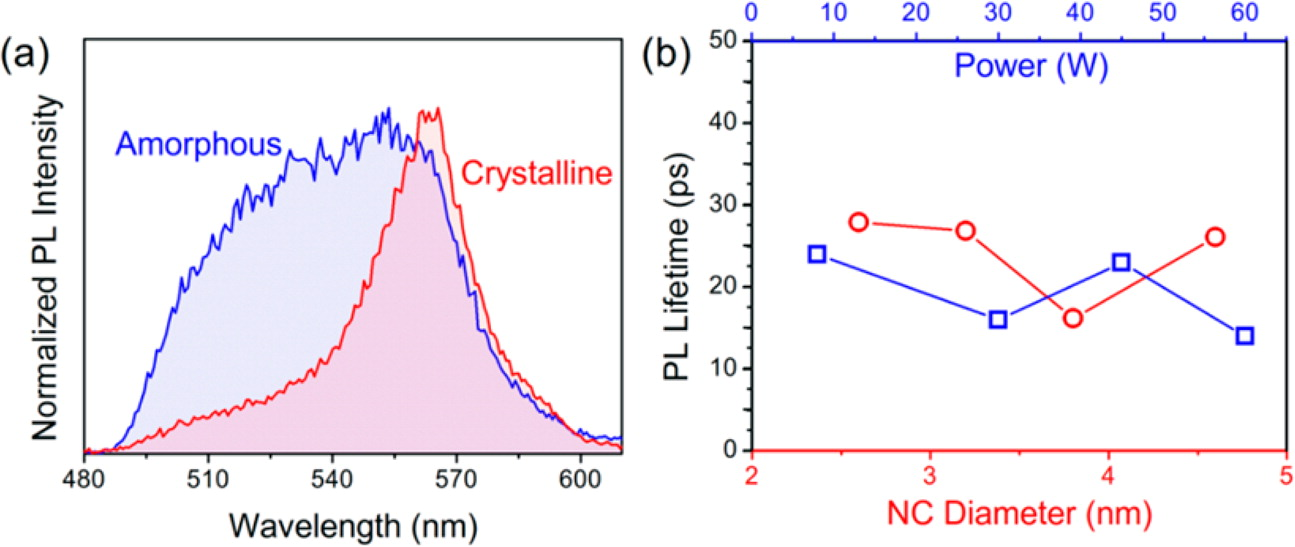
\includegraphics[width=\textwidth]{./Chapter6/amsi4.jpeg}
\caption[Comparison of PL from crystalline and amorphous Si NPs.]{(a) Mathematically normalized PL spectra temporally binned from 0-100 ps following photoexcitation for Si NPs synthesized for amorphous (8 W) and crystalline (60 W) Si NPs, which are indicated on the figure. Although filtering optics artificially truncate the red edge of the PL spectrum, the same optics were used in collection of both PL spectra displayed. (b) Lifetime of the fastest dynamics observed for all of the samples considered in this study. The blue (squares) data and top axis correspond to the Si NPs synthesized at indicated plasma powers, while the red (circles) data and bottom axis correspond to four sizes of highly crystalline Si NPs.}
\label{f:amsi4}
\end{center}
\end{figure}

We aim to resolve the origin of blue PL photons emitted from Si NPs as well as the processes responsible for the decay of the associated PL band (the blue feature). Regarding the dynamics of the blue PL feature, we note that the NP size-independent fastest PL decay of $\sim$30 ps is an order of magnitude slower than typical intraband relaxation time in quantum-confined materials \cite{PhysRevLett.80.4028,PhysRevLett.95.196401}, a process with which phononless PL would be competitive. Conversely, if indeed the rapid PL decay were associated with hot carrier recombination, it would imply the slowest intraband relaxation time ever reported for core-only colloidal NPs. Furthermore, the red PL feature, which we recently established arises from lowest-energy exciton states within the NP core \cite{hannah2012origin}, does not exhibit a rise time that correlates with the “green” feature decay (as observable at 525 nm in Figure \ref{f:amsi2}(a)), consistent with ultrafast (1 ps or less) relaxation of hot excitons as found in numerous other semiconductor NPs \cite{PhysRevLett.80.4028,PhysRevLett.95.196401}. This lack of a correlated rise time offers additional evidence that the $\sim$30 ps decay does not represent a hot exciton radiative process. \par

Instead, we posit that the $\sim$30 ps decay feature arises from a nonradiative process associated with amorphous material. Indeed, if a radiative process were responsible, the biexponential dynamics would imply two separate populations of emitters with different associated PL line widths. Given the unchanging PL profile (Figure \ref{f:amsi2}(b)), it is unlikely that biexponential dynamics arise from two separate radiating populations. This notion is further supported by the absence of a strong optical absorption transition in this spectral region \cite{gresback2011combined}. Considering the oscillator strength, which would be associated with such a rapid radiative transition, it is highly unlikely that a 30 ps decay (which represents the upper bound of our lifetime measurements) caused by optical transitions would have no apparent manifestation in the optical absorption spectrum of the Si NPs. Fermi's Golden Rule allows us to relate the optical radiative rate ($\tau_{PL}^{-1}$) to the optical transition matrix element $|\left\langle\Psi_1|\vec{p}|\Psi_0\right\rangle|^2$ \emph{via} Eq. \ref{eq:amsi1}:

\begin{equation}\label{eq:amsi1}
\tau_{PL}^{-1} = \frac{e^2n\omega}{\pi\varepsilon_0m^2\hbar c^3}|\left\langle\Psi_1|\vec{p}|\Psi_0\right\rangle|^2
\end{equation}

In Eq. \ref{eq:amsi1}, $e$ is the fundamental charge, $n$ is the refractive index, $\hbar\omega$ is the emission energy, $\varepsilon_0$ is the vacuum permittivity, $m$ is the electron mass, and $c$ is the speed of light in vacuum.  Coupled with the expression for oscillator strength ($f = (2/\hbar m\omega)|\left\langle\Psi_1|\vec{p}|\Psi_0\right\rangle|^2$), we can express the oscillator strength of a given transition in terms of radiative lifetime, as shown in Eq. \ref{eq:amsi2}:

\begin{equation}\label{eq:amsi2}
f = \frac{2\pi\varepsilon_0mc^3}{e^2n\omega^2}\frac{1}{\tau_{PL}}
\end{equation}

For the 30 ps decay ($\hbar\omega = 2.75$ eV, $\tau_{PL}$ = 30 ps), a radiative transition would be associated with an oscillator strength of $f = 13.8$.  By comparison, the long-lived red PL ($\hbar\omega = 1.75$ eV, $\tau_{PL} = 75$ $\mu$s) has an oscillator strength of $f = 1.3 \times 10^{-5}$, which is several orders of magnitude smaller. Provided that significant silicon atom rearrangements do not occur in the excited state, the absence of a strong optical transition near 450 nm in the absorption spectrum taken together with the constant PL line width (Figure \ref{f:amsi2}(b)) strongly suggest that radiative recombination cannot account for the $\sim$30 ps decay observed here. \par

Recently, Dohnalova and co-workers suggested an intrinsic origin to the blue band observed for alkyl-terminated Si NPs prepared \emph{via} a wet chemical synthesis \cite{dohnalova2013surface}. For these NPs, they report primarily blue PL and an absence of red emission, suggesting that the blue band is not related to hot exciton emission (a scenario in which one would expect to see blue and band-edge red PL). Following intense laser irradiation they observe an increase of red PL, which they attribute to sample oxidation. However, their results may also be interpreted in the context of our work as arising from changes in sample crystallinity. The wet chemical synthesis used in the study by Dohnalova \emph{et al.} may not have provided sufficient energy to form c-Si, a covalently bonded material. Upon laser irradiation, we suggest that sample annealing occurs, increasing the amount of crystalline material present and, consequently, the relative intensity of the red PL, which we and others attribute to indirect gap, band-edge recombination. Similarly, a recent study by Dasog and co-workers found that Si NPs synthesized at higher temperatures exhibited red, indirect gap PL, while Si NPs synthesized \emph{via} more mild colloidal routes yielded rapid, blue PL \cite{dasog2013chemical}. These results, taken in conjunction with our presented data, lead us to the conclusion that high-energy PL is a result of emission arising from amorphous material. The persistence of amorphous material even in our most crystalline samples is supported by near-exact agreement between experimental Raman scattering spectra for c-Si NPs and theoretical Raman spectra calculated for crystalline core particles covered by a two-monolayer amorphous shell. The presence of amorphous material in the form of a persistent shell is supported by our observation of a disordered surface layer in TEM images as well as the presence of SiHi$_3$ and SiH$_2$ on the NP surface (see Appendix C). \par

In addition to the spectral similarities noted above for amorphous Si NPs and the blue feature observed in crystalline Si NPs, we find that PL dynamics for amorphous Si strongly resemble those found for the blue feature in crystalline Si. Indeed, regardless of sample size or crystallinity, we find the fastest PL decay observed to have a time constant of $\sim$30 ps. This is depicted in Figure \ref{f:amsi4}(b), which shows the fitted time constant obtained for the fastest decay in the system for each sample considered in this study. The similarity and time scale of these dynamics suggests that in all cases, rapid PL decay is caused by the same (nonradiative) process. Furthermore, the longer component of the blue PL decay, for each power used, has a fitted time constant between 150 and 200 ps, very similar to the highly crystalline Si NPs studied in this work (Table 1). The rapid decay process we observe in completely amorphous (8 W) Si NPs is likely hole trapping in the strained regions of the amorphous network. This type of trapping was suggested in recent theoretical works by Lajoie \emph{et al}. \cite{lajoie2010optical} and Wagner \emph{et al.} \cite{wagner2008microscopic}. Given that a multitude of characterization methods (TEM, FTIR, Raman) indicate that highly crystalline particles still present an amorphous surface layer, we suggest that hole trapping processes occur in this thin amorphous shell. \par

\subsubsection{Conclusions}
Overall, we have identified and resolved, in the energy and time domains, a high energy (400-600 nm) band in the PL spectrum of plasma-synthesized, covalently functionalized Si NPs. Our findings constitute a comprehensive examination of the ultrafast dynamics of the 400-to-600 nm PL band previously attributed to both defect-related recombination and phononless PL in Si NPs. Whereas previous reports noted instrumentation-limited decay features, we examine these features with instruments having a response time adequate to resolve them. This new information allows us to resolve long-standing controversies regarding the fast PL band in quantum confined Si and conclusively attribute observed dynamics to a nonradiative decay process which we suggest is hole trapping in a persistent surface layer of amorphous Si. For the first time, we also examine the role of core crystallinity in PL. These results shed light on the origin of high energy PL in Si NPs and also provide an explanation for the observation of this PL in a wide variety of Si NP preparations, as they do not invoke surface chemistry or pseudodirect gap recombination. We expect that our work will stimulate future experimental and theoretical efforts regarding the role of lattice disorder in the optical properties of silicon nanomaterials. Furthermore, these findings present an opportunity for the systematic tailoring of absorption and emission spectra \emph{via} core crystallinity, providing an additional degree of tunability to this technologically important class of materials.
